\def\year{2019}\relax
%File: formatting-instruction.tex
\documentclass[letterpaper]{article} % DO NOT CHANGE THIS
 \usepackage{booktabs}
\usepackage{aaai19}  % DO NOT CHANGE THIS
\usepackage{times}  % DO NOT CHANGE THIS
\usepackage{helvet} % DO NOT CHANGE THIS
\usepackage{courier}  % DO NOT CHANGE THIS
\usepackage[hyphens]{url}  % DO NOT CHANGE THIS
\usepackage{graphicx} % DO NOT CHANGE THIS
\urlstyle{rm} % DO NOT CHANGE THIS
\def\UrlFont{\rm}  % DO NOT CHANGE THIS
\usepackage{graphicx}  % DO NOT CHANGE THIS
\frenchspacing  % DO NOT CHANGE THIS
\setlength{\pdfpagewidth}{8.5in}  % DO NOT CHANGE THIS
\setlength{\pdfpageheight}{11in}  % DO NOT CHANGE THIS
\usepackage{multirow}
\usepackage{acronym}
\usepackage{xspace}
\acrodef{MAPF}{Multi-Agent Pathfinding}
\acrodef{SOC}{Sum-of-Costs}
\newcommand{\mapf}{\ac{MAPF}\xspace}
\newcommand{\soc}{\ac{SOC}\xspace}
\newcommand{\tuple}[1]{\ensuremath{\left \langle #1 \right \rangle }}


%PDF Info Is REQUIRED.
% For /Author, add all authors within the parentheses, separated by commas. No accents or commands.
% For /Title, add Title in Mixed Case. No accents or commands. Retain the parentheses.
% /Title ()
% Put your actual complete title (no codes, scripts, shortcuts, or LaTeX commands) within the parentheses in mixed case
% Leave the space between \Title and the beginning parenthesis alone
% /Author ()
% Put your actual complete list of authors (no codes, scripts, shortcuts, or LaTeX commands) within the parentheses in mixed case.
% Each author should be only by a comma. If the name contains accents, remove them. If there are any LaTeX commands,
% remove them.

% DISALLOWED PACKAGES
% \usepackage{authblk} -- This package is specifically forbidden
% \usepackage{balance} -- This package is specifically forbidden
% \usepackage{caption} -- This package is specifically forbidden
% \usepackage{color (if used in text)
% \usepackage{CJK} -- This package is specifically forbidden
% \usepackage{float} -- This package is specifically forbidden
% \usepackage{flushend} -- This package is specifically forbidden
% \usepackage{fontenc} -- This package is specifically forbidden
% \usepackage{fullpage} -- This package is specifically forbidden
% \usepackage{geometry} -- This package is specifically forbidden
% \usepackage{grffile} -- This package is specifically forbidden
% \usepackage{hyperref} -- This package is specifically forbidden
% \usepackage{navigator} -- This package is specifically forbidden
% (or any other package that embeds links such as navigator or hyperref)
% \indentfirst} -- This package is specifically forbidden
% \layout} -- This package is specifically forbidden
% \multicol} -- This package is specifically forbidden
% \nameref} -- This package is specifically forbidden
% \natbib} -- This package is specifically forbidden -- use the following workaround:
% \usepackage{savetrees} -- This package is specifically forbidden
% \usepackage{setspace} -- This package is specifically forbidden
% \usepackage{stfloats} -- This package is specifically forbidden
% \usepackage{tabu} -- This package is specifically forbidden
% \usepackage{titlesec} -- This package is specifically forbidden
% \usepackage{tocbibind} -- This package is specifically forbidden
% \usepackage{ulem} -- This package is specifically forbidden
% \usepackage{wrapfig} -- This package is specifically forbidden
% DISALLOWED COMMANDS
% \nocopyright -- Your paper will not be published if you use this command
% \addtolength -- This command may not be used
% \balance -- This command may not be used
% \baselinestretch -- Your paper will not be published if you use this command
% \clearpage -- No page breaks of any kind may be used for the final version of your paper
% \columnsep -- This command may not be used
% \newpage -- No page breaks of any kind may be used for the final version of your paper
% \pagebreak -- No page breaks of any kind may be used for the final version of your paperr
% \pagestyle -- This command may not be used
% \tiny -- This is not an acceptable font size.
% \vspace{- -- No negative value may be used in proximity of a caption, figure, table, section, subsection, subsubsection, or reference
% \vskip{- -- No negative value may be used to alter spacing above or below a caption, figure, table, section, subsection, subsubsection, or reference

\usepackage{tikz}
\usetikzlibrary{arrows.meta,shapes}
\usepackage{color}

%
% Add comments in the text
%
\usepackage{soul}
\usepackage{float}
\usepackage{graphicx}
\usepackage{xspace}
\usepackage[utf8]{inputenc}
\usepackage[small]{caption}
\usepackage{amsmath}
\usepackage{amsthm}
\usepackage{amssymb}
\usepackage{ifthen}

\newboolean{showcomments}
%\setboolean{showcomments}{true}
\setboolean{showcomments}{false}

\ifthenelse{\boolean{showcomments}}
  {\newcommand{\nb}[3]{
  {\color{#2}\small\fbox{\bfseries\sffamily\scriptsize#1}}
  {\color{#2}\sffamily\small$\triangleright~$\textit{\small #3}$~\triangleleft$}
  }
  }
  {\newcommand{\nb}[3]{}
  }

\newcommand\Roni[1]{\nb{\textbf{Comment:}}{orange}{#1}}


\newcommand{\comment}[1]{{\nb{\textbf{Comment:}}{orange}{#1}}}
\setcounter{secnumdepth}{2} %May be changed to 1 or 2 if section numbers are desired.

% The file aaai19.sty is the style file for AAAI Press
% proceedings, working notes, and technical reports.
%
\setlength\titlebox{2.5in} % If your paper contains an overfull \vbox too high warning at the beginning of the document, use this
% command to correct it. You may not alter the value below 2.5 in
\title{Multi-Agent Pathfinding: Definitions, Variants, and Benchmarks}
%Your title must be in mixed case, not sentence case.
% That means all verbs (including short verbs like be, is, using,and go),
% nouns, adverbs, adjectives should be capitalized, including both words in hyphenated terms, while
% articles, conjunctions, and prepositions are lower case unless they
% directly follow a colon or long dash
%\author{Written by AAAI Press Staff\textsuperscript{\rm 1}\thanks{Primarily Mike Hamilton of the Live Oak Press, LLC, with help from the AAAI Publications Committee}\\ \Large \textbf{AAAI Style Contributions by Pater Patel Schneider,} \\ \Large \textbf{Sunil Issar, J. Scott Penberthy, George Ferguson, Hans Guesgen}\\ % All authors must be in the same font size and format. Use \Large and \textbf to achieve this result when breaking a line \textsuperscript{\rm 1}Association for the Advancement of Artificial Intelligence\\ %If you have multiple authors and multiple affiliations
% use superscripts in text and roman font to identify them. For example, Sunil Issar,\textsuperscript{\rm 2} J. Scott Penberthy\textsuperscript{\rm 3} George Ferguson,\textsuperscript{\rm 4} Hans Guesgen\textsuperscript{\rm 5}. Note that the comma should be placed BEFORE the superscript for optimum readability 2275 East Bayshore Road, Suite 160\\ Palo Alto, California 94303\\ publications19@aaai.org % email address must be in roman text type, not monospace or sans serif }

\author{
Roni Stern,\textsuperscript{\rm 1}
Nathan R. Sturtevant,\textsuperscript{\rm 2}
Ariel Felner,\textsuperscript{\rm 1}
Sven Koenig,\textsuperscript{\rm 3}
Hang Ma,\textsuperscript{\rm 3}\\
\bf \Large Thayne T. Walker,\textsuperscript{\rm 4}
Jiaoyang Li,\textsuperscript{\rm 3}
Dor Atzmon,\textsuperscript{\rm 1}
Liron Cohen,\textsuperscript{\rm 3}
T. K. Satish Kumar,\textsuperscript{\rm 3}
Eli Boyarski,\textsuperscript{\rm 1}
Roman Bart\'{a}k\textsuperscript{\rm 5} \\
\textsuperscript{\rm 1}Ben Gurion University of the Negev,
\textsuperscript{\rm 2}University of Alberta,
\textsuperscript{\rm 3}USC,
\textsuperscript{\rm 4}University of Denver
\textsuperscript{\rm 5}Charles University\\
sternron@post.bgu.ac.il,
nathanst@ualberta.ca,
felner@bgu.ac.il,
skoenig@usc.edu,
hangma@usc.edu,
thayne.walker@du.edu,\\
jiaoyanl@usc.edu,
dorat@post.bgu.ac.il,
lironcoh@usc.edu,
tkskwork@gmail.com,
boyarske@post.bgu.ac.il,
bartak@ktiml.mff.cuni.cz
}
%\author{\name Roni Stern \email sternron@post.bgu.ac.il\\
%        \name Nathan R. Sturtevant \email nathanst@ualberta.ca \\
%        \name Ariel Felner \email felner@bgu.ac.il \\
%        \name Sven Koenig \email skoenig@usc.edu \\
%        \name Hang Ma \email hangma@usc.edu\\
%        \name Thayne Walker \email thayne.walker@du.edu\\
%        \name Jiaoyang Li \email jiaoyanl@usc.edu\\
%        \name Dor Atzmon \email dorat@post.bgu.ac.il\\
%        \name Liron Cohen \email lironcoh@usc.edu\\
%        \name T. K. Satish Kumar \email tkskwork@gmail.com\\
%        \name Eli Boyarski \email boyarske@post.bgu.ac.il\\
%        \name Please add your names also\email your@mail\\}
%\author{Submission \#56}

 \begin{document}

\maketitle

\begin{abstract}	The \mapf problem is the fundamental problem of planning paths for multiple agents, where the key constraint is that the agents will be able to follow these paths concurrently without colliding with each other. Applications of \mapf include automated warehouses and autonomous vehicles. Research on \mapf has been flourishing in the past couple of years.
	Different \mapf research papers make different assumptions, e.g., whether agents can traverse the same road at the same time, and have different objective functions, e.g., minimize makespan or sum of agents' actions costs.
	These assumptions and objectives are sometimes implicitly assumed or described informally. This makes it difficult to establish appropriate baselines for comparison in research papers, as well as making it difficult for practitioners to find the papers relevant to their concrete application.
	This paper aims to fill this gap and support researchers and practitioners by providing a unifying terminology for describing common \mapf assumptions and objectives. In addition, we also provide pointers to two \mapf benchmarks. In particular, we introduce a new grid-based benchmark for \mapf, and demonstrate experimentally that it poses a challenge to contemporary \mapf algorithms.
\end{abstract}


\section{Introduction}

% Brief: what is MAPF
\mapf is an important type of multi-agent planning problem in which the task is to plan paths for multiple agents,
where the key constraint is that the agents will be able to follow these paths concurrently without colliding with each other. \mapf has a range of relevant contemporary applications including automated warehouses, autonomous vehicles, and robotics. Consequently, this problem has received attention in recent years from various research groups and academic communities~\cite{standley2010finding,felner2017search,surynek2016empirical,bartak2018aScheduling,cohen2018anytime,li2019multi,MaAAAI19a}.

% The challenge: different variants and terminology
Different \mapf research papers consider different sets of assumptions about the agents and aim for different objectives. These assumptions and objectives are sometimes implicitly assumed or described informally. Even in cases where the assumptions and objective function are described formally, there are still differences in used \mapf terminology. This makes it difficult to navigate through and understand existing literature and to establish appropriate baselines for comparison. In addition, it makes it difficult for practitioners to find papers relevant to their concrete application.

This paper aims to address this growing challenge by introducing  a \textbf{unified terminology} to describe \mapf problems, and by establishing \textbf{common benchmarks and evaluation measures} for evaluating \mapf algorithms.
% Unified terminology
The unified \mapf terminology we present in this paper is our attempt to classify the currently studied  \mapf variants. We hope this terminology will serve as a common ground for future researchers, and will be used by them to describe their contributions succinctly and accurately. %, and similarly enable practitioners to describe and find the MAPF research that fits their needs.

% Shared benchmarks and evaluation measures
In the second part of this paper, we introduce a new grid \mapf benchmark to the community. This benchmark includes a diverse set of maps, as well as generated source and target vertices. We report the performance of a standard \mapf algorithm on this benchmark, to serve as baseline for comparison to future research. This benchmark is intended to help future researchers and enable more scientifically rigorous empirical comparisons of existing and future \mapf algorithms. We do not claim that these benchmarks are perfect, as they may have some biases. But, through their use and study these biases can be discovered and corrected. It is also important to emphasize that this document is not intended to be a survey of  state of the art MAPF algorithms. For such a survey, see~\cite{felner2017search,ma2017buzz}.
In addition, the newly created website
\url{http://mapf.info} contains \mapf-related tutorials and other resources.

%\comment{Roni: To all: please feel free to add here your favorite survey of MAPF, including your own work}



\section{Classical MAPF}
We first describe what we refer to as a \emph{classical MAPF} problem.
The input to a classical MAPF problem with $k$ agents is
a tuple $\langle G, s, t\rangle$
where $G=(V,E)$ is an undirected graph,
$s:[1,\ldots,k]\rightarrow V$ maps an agent to a source vertex,
and $t:[1,\ldots,k]\rightarrow V$ maps an agent to a target vertex.
% Time and actions
Time is assumed to be discretized, and in every time step each agent is situated in one of the graph vertices
and can perform a single \emph{action}.
An action in classical MAPF is a function $a: V\rightarrow V$
such that $a(v)=v'$ means that if an agent is at vertex $v$ and performs $a$ then it will be in vertex $v'$ in the next time step.
Each agent has two types of actions: \emph{wait} and \emph{move}.
A \emph{wait} action means that the agent stays in its current vertex another time step.
% Formally, a wait action is the identity function $a(v)=v$.
A \emph{move} action means that the agent moves from its current vertex $v$ to an adjacent vertex $v'$ in the graph (i.e., $(v,v')\in E$).
% Formally, for every edge $e=(v,v')$ there is a move action $a(v)=v'$.

% A solution to a MAPF problem
For a sequence of actions $\pi=(a_1,\ldots a_n)$
and an agent $i$,
we denote by $\pi_i[x]$
the location of the agent after executing  the first $x$ actions in $\pi$, starting from the agent's source $s(i)$.
Formally, $\pi_i[x]=a_x(a_{x-1}(\cdots a_1(s(i))))$.
A sequence of actions $\pi$ is a \textbf{single-agent plan} for agent $i$ iff executing this sequence of actions in $s(i)$ results in being at $t(i)$,
that is, iff $\pi_i[|\pi|]=t(i)$.
A \textbf{solution} is a set of $k$ single-agent plans, one for each agent.
%\comment{Ariel: t serves both for time and for target. This is confusing. Maybe change target to goal}
%\comment{Roni: I changed t to x for marking time}
%We highlight the simplifying assumptions made in the classical MAPF setting:
%\begin{itemize}
%    \item Actions are atomic.
%    \item Time is discretized.
%\end{itemize}


\subsection{Types of Conflicts in Classical MAPF}

%Single-agent plans may \emph{conflict}, and a key constraint in MAPF is to a that s
%[[AF: above you defnied a solution as a set of singile agent plans. Here you define it as a plan. Try to use one term only]][[Roni: it is consistent: we want to find a solution. A solution is  set of plans. So, we want ot find plans]
The overarching goal of MAPF solvers is to find a solution, i.e., a single-agent plan for each agent, that can be executed without collisions. To achieve this, MAPF solvers use the notion of \emph{conflicts} during planning, where a MAPF solution is called \emph{valid} iff there is no conflict between any two single-agent plans. The definition of what constitutes a conflict depends on the environment, and correspondingly the literature on classical MAPF includes several different definitions of what constitutes a conflict between plans. We list common conflict definitions below. Let $\pi_i$ and $\pi_j$ be a pair of single-agent plans.

%\comment{Thayne: added definition of "feasibility rule" here and added "k-robustness" as an additional feasibility rule in section 3}\comment{Roni: I moved the feasiblity rule part to the later section you added, as I felt it over-complicated things here. }



\begin{itemize}
\item \textbf{Vertex conflict.} A \emph{vertex conflict} between $\pi_i$ and $\pi_j$ occurs iff  according to these plans the agents are planned to occupy the same vertex at the same time step.
Formally, there is a vertex conflict between $\pi_i$ and $\pi_j$ iff there exists a time step $x$ such that
$\pi_i[x]=\pi_j[x]$.
%Note that if there is an edge conflict between plans, then these plans must also have at least two vertex conflicts.

\item \textbf{Edge conflict.} An \emph{edge conflict} between $\pi_i$ and $\pi_j$ occurs iff
according to these plans the agents are planned to traverse the same edge at the same time step in the same direction.
Formally, there is an edge conflict between $\pi_i$ and $\pi_j$ iff there exists a time step $x$ such that
$\pi_i[x]=\pi_j[x]$ and $\pi_i[x+1]=\pi_j[x+1]$.
%\comment{Liron: This definition simply describes two vertex conflicts. Do we really need it or do I miss something? And, if we decide to keep it, how about the name ``durative'' conflict (that way we can keep edge conflict to what it normally means).}\comment{Roni: yes, but there is an "AND" between these conflicts. That is, we say that there is an edge conflict iff there is a vertex conflict in both end points of the same edge. So, it is more restrictive than a single vertex conflict.}



\item \textbf{Following conflict.} A \emph{following} conflict between $\pi_i$ and $\pi_j$ occurs iff
one agent is planned to occupy a vertex that was occupied by another agent in the previous time step.
Formally, there is a following conflict between $\pi_i$ and $\pi_j$ iff there exists a time step $x$ such that
$\pi_i[x+1]=\pi_j[x]$.

%\comment{Nathan: There are two types of these. In one type all agents are moving the same direction - this is always physically feasible. If agents are moving at 90$^{\circ}$ angles this might not always be feasible.}
%\comment{Roni: I was aiming here for the first type, as I think it is the more common constraint, resulting in a pebble-like movement. The second type is a special case of collision between actions. I'll write something about that later}

\item \textbf{Cycle conflict.} A \emph{cycle} conflict  between a set of single-agent plans $\pi_i, \pi_{i+1}, \ldots \pi_j$ occurs iff
in the same time step every agent moves to a vertex that was previously occupied by another agent, forming a ``rotating cycle'' pattern. Formally, a \emph{cycle conflict} between a set of plans $\pi_i, \pi_{i+1}, \ldots \pi_j$
occurs iff there exists a time step $x$ in which
$\pi_i(x+1)=\pi_{i+1}(x)$
and $\pi_{i+1}(x+1)=\pi_{i+2}(x)$
$\ldots$
and $\pi_{j-1}(x+1)=\pi_j(x)$
and $\pi_j(x+1)=\pi_i(x)$.


\item \textbf{Swapping conflict.} A \emph{swapping} conflict between $\pi_i$ and $\pi_j$ occurs iff
the agents are planned to swap locations in a single time step.
Formally, there is a swapping conflict between $\pi_i$ and $\pi_j$ iff there exists a time step $x$ such that
$\pi_i[x+1]=\pi_j[x]$ and $\pi_j[x+1]=\pi_i[x]$. This conflict is sometimes called \emph{edge conflict} in the current \mapf literature.

%Note that if there is a swapping conflict between plans, then these plans must also have at least two following conflicts.
%\comment{Ariel: isn't this an edge conflict?}
%\comment{Nathan: The problem is defined as a directed graph, in which case this wouldn't be the same edge. For the {\em classical} problem isn't the graph undirected?}
%\comment{Roni: following both of your comments, I defined an edge conflict earlier,  renamed this to ``swapping'' conflict,  and have it consider the vertices in the plan and not the edges.  I don't think we need to assume an undirected graph even in the classical setting,  but I do think it makes sense to define that there is at most one edge between two pairs of vertices.  I wonder if this needs to be said explicitly, or does this come with the definition of a graph. Any thoughts on this?}
%\comment{Liron: I agree with Ariel - it seems like swapping conflict is called edge conflict in many other papers.}
%\comment{Roni: I agree, but I think this is a source for confusion -- when one says "edge conflict" does one implicitly mean an undirected graph? does one allow swapping? and so on. So, I think the definitions above are cleaner, and this is a good opportunity to clean things. Opinions?}
\end{itemize}

\begin{figure}
    \centering
    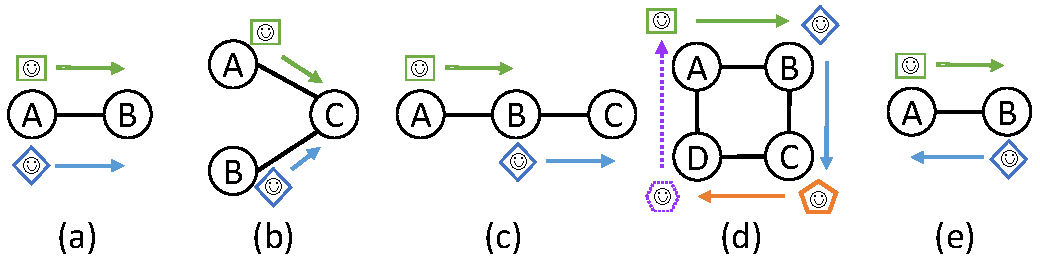
\includegraphics[width=\columnwidth]{types-of-conflicts.pdf}
    \caption{An illustration of common types of conflicts. From left to right: an edge conflict, a vertex conflict, a following conflict, a cycle conflict, and a swapping conflict.}
    \label{fig:types-of-conflicts}
\end{figure}

%\comment{Roni: TODO: Draw a nice example to demonstrate the different types of conflicts}
Figure~\ref{fig:types-of-conflicts} illustrates the different types of conflicts. Note that the above set of conflict definitions is certainly not a complete set of all possible conflicts.
Considering the formal definitions of these conflicts, it is clear that there are dominance relation between them: (1) forbidding vertex conflicts implies edge conflicts are also forbidden, (2) forbidding following conflicts implies cycle conflicts and swapping conflicts are also forbidden, (3) forbidding cycle conflicts implies that swapping conflicts are also forbidden. Vice versa, (1) allowing edge conflicts implies vertex conflicts are also allowed,
(2) allowing swapping conflicts implies cycle conflicts are also allowed,\footnote{A swapping conflict is, in fact, a cycle conflict for two agents.}
and (3) allowing cycle conflicts implies following conflicts are also allowed.


%In addition, some conflicts can be defined with respect to a set of more than two plans.  For example, one can allow following conflicts but only if the leading agent moves to an empty vertex.  That is, to forbid any set of agents from ``rotating'' in a cyclic pattern. Formally,  such a \emph{cycle conflict} between a set plans $\pi_i, \pi_{i+1}, \ldots \pi_j$  occurs if there exists a time step $x$ in which  $\pi_i(x+1)=\pi_{i+1}(x)$   and $\pi_{i+1}(x+1)=\pi_{i+2}(x)$  $\ldots$  and $\pi_{j-1}(t+1)=\pi_j(x)$  and $\pi_j(x+1)=\pi_i(x)$.

%\comment{Roni: there is another type of conflict that Ariel mentioned in a comment  (and I also got in a review). This conflict talks about a cyclic form of the ``following'' conflict.  This conflict occurs between  a set plans $\pi_i, \pi_{i+1}, \ldots \pi_j$ if all the agents following these plans end up rotating locations. Formally, there is a cyclic conflict between a set plans $\pi_i, \pi_{i+1}, \ldots \pi_j$  if there exists a time step $t$ in which  $\pi_i(t+1)=\pi_{i+1}(t)$   and $\pi_{i+1}(t+1)=\pi_{i+2}(t)$  $\ldots$  and $\pi_{j-1}(t+1)=\pi_j(t)$  and $\pi_j(t+1)=\pi_i(t)$.  Note that if there is this following-cycle conflict between $n$ plans then  these set of plans have at least $n$ following conflicts between them.  I did not add this conflict above since I am not familiar with prior work that  allowed following conflicts but did not allow this cyclic-following conflict. So, I wonder if we're just inventing a variant that no one cares about. What do you think?}
%\comment{Liron: General comment for this section, I wonder if grounding the discussion on conflicts in the ``physical'' world will be helpful (especially for cycle conflicts or following conflicts)? What we really want is to be able to execute plans on robots (or game figures, etc.) with the guarantee that robots will not collide with each other. To achieve this, MAPF solvers use the notion of conflicts during planning. The definition of what constitutes a conflict many times boil down to how the environment (and time) is discretized and how actions (/time) are synchronized.}
%\comment{Roni: I like this view, and took some of your text up to the intro of this section. Hope this captures your intention}


% Relation to current work
%\comment{Roni: I think that throughout the paper we should refer to existing papers that assume the different assumptions. This well help reader orientation, but also focus us to not introduce every possible variant of MAPF we can think of. I added such a paragraph for classical MAPF below. }
To properly define a classical MAPF problem, one needs to specify which types of conflicts are allowed in a solution.
The least constrained restriction is to only forbid edge conflicts.
However, to the best of our knowledge,
all prior work on classical MAPF also forbid vertex conflicts. Some work on MAPF with payload transfers allows swapping conflicts~\cite{MaAAAI16}.
Most work on search-based MAPF algorithms~\cite{standley2010finding,felner2017search} forbid swapping conflicts, but allow following conflicts.
Some work on compilation-based MAPF algorithms
as well as all work that consider MAPF as a pebble motion problem, forbid following conflicts as well~\cite{surynek2016empirical,bartak2017modeling}.
%\comment{Roni: Anyone has a nice reference to add here for this?}


%A solution to a MAPF problem is called \emph{valid} if the only conflicts that exist between its constituent single-agent plans, if any, are allowed. \comment{Roni: the last sentence is a bit clumsy. TODO: Find a better phrasing} [[AF: If it is allowed, it is not a conflict. I think we should define what is allowed for agents. Then, discuss conflicts. See my next subsection. Needs to be decided]][[Roni: I rephrased all the above to make it cleaner.]

\subsection{Agent Behavior at Target in Classical MAPF}

In a solution to a classical MAPF problem,
agents may reach their targets at different time steps.
Therefore, when defining a classical MAPF problem one must define
how an agent behaves in the time steps after it has reached its target and before the last agent has reached its target.

There are two common assumptions for how agents behave at their targets.
\begin{itemize}
\item \textbf{Stay at target} Under this assumption,
an agent waits in its target until all agents have reached their targets.
This waiting agent will cause a vertex conflict with any plan that passes through
its target after it has reached it.
Formally, under the stay-at-target assumption,
a pair of single-agent plans $\pi_i$ and $\pi_j$ will have a vertex conflict
if there exists a time step $t\geq |\pi_i|$ such that $\pi_j[t]=\pi_i[|\pi_i|]$.
\item \textbf{Disappear at target} Under this assumption,
when an agent reaches its target it immediately disappears.
This means the plan of that agent will not have any conflict after
the time step in which the corresponding agent has reached its target.
\end{itemize}
Most prior work on classical MAPF assumed stay-at-target, but recent work also considered the disappear-at-target assumption~\cite{MaAAAI19a}.
%\comment{Roni: all my work has been under the stay-at-goal assumption (except online MAPF, which certainly does not fall under the category of classical MAPF). Anyone familiar with prior work on classical MAPF that assumed disappear-at-goal?}
%\comment{Jiaoyang: \cite{MaAAAI19a} has experimented on some MAPF instances that assumed disappear-at-goal.}
%\comment{Roni: Thanks! I added the line above to capture this.}

\subsection{Objective Functions in Classical MAPF}
It is safe to say that in most real applications of MAPF,
some MAPF solutions are better than others.
To capture that, work in classical MAPF considers an \textbf{objective function}
that is used to evaluate MAPF solutions.
The two most common functions used for evaluating a solution in classical MAPF are \emph{makespan} and \emph{sum of costs}.
\begin{itemize}
\item \textbf{Makespan.} The number of time steps required for all agents to reach their target.
For a MAPF solution $\pi=\{\pi_1, \ldots \pi_k\}$, the makespan of $\pi$ is defined as $\max_{1\leq i\leq k} |\pi_i|$.
\item \textbf{Sum of costs.} The sum of time steps required by each agent to reach its target. The sum of costs of $\pi$ is defined as $\sum_{1\leq i\leq k} |\pi_i|$.
Sum of costs is also known as \emph{flowtime}.
\end{itemize}


% \item \textbf{Sum of fuel.} The total non-waiting actions required to reach the goal. We sum this over all agents. \item \textbf{Sum of time off goal.} The time spent by the agent not in the goal location. We sum this over all agents. \item \textbf{Time before final reach of goal.} The time spent by the agent until it reached its goal for the last time. For example, assume that an agent reached its goal at $t_1$ but then moved away at $t_2$ and arrived again at the goal at time $t_3$ and stayed there forever. Its cost is therefore $t_3$. By contrast, the {\em Time off goal} variant will incur a cost of $t_1$ + $t_3 - t_2$.[[AF: Guni used this variant in many of his experiments.]] We note that the aggregated cost of this variant is not consistent. Because when the agent moves away at $t_2$ its cost jumps right away from $t_1$ to $t_2$. [[AF: This is why I hated this variant all those years, but Guni liked it]]
%\item \textbf{Makespan then sum of costs} Among all solutions with the same makespan, choose the one with the lowest sum-of-costs. [[Eli: Pavel uses this one, at least in one paper]]
%\end{itemize}

If the agent-at-target behavior is \emph{stay at target} and the objective function is \emph{sum of costs}, then one needs to specify how  staying at a target affects the sum of costs. For example, one can define that, if an agent waits at its target, then it does not increase the sum of costs. The common assumption in most prior work is that an agent staying in its target counts as a wait action unless it is not planning to move away from its target again. For example, assume that agent $i$ reaches its target at time step $t$, leaves its target at time step $t'$, arrives back at its target at time step $t''$,
and then stays at its target until all agents reach their target.
Then, this single-agent plan will contribute $t''$ to the sum of costs of the corresponding solution.
%[[AF: I like this as this only counts time steps that the agent was outside its goal and the cost function is monotonically increasing and consistent]][[Roni: all cost functions are monotonic non-decreasing, but I agree that consistency is nice.]]
%\comment{Roni: I am not sure we need all the above paragraph. Are you familiar with any prior work in which waiting at the goal is free? if we follow our definition of sum-of-cost to the letter, then all the above paragraph is redundant. AF: I think it is important. I think that we should have always used the "you incur cost anytime you are outside the goal". It makes more sense to me and is more elegant]]}\roni{Ok, so I left it there}
%[[AF: see my last item]]

%\comment{Roni: Again, I added the paragraph below to connect all the above definitions to real papers and prior work}
We do not claim that these are the only possible objective functions for classical MAPF.
One may define other objective functions, such as the total non-waiting actions required to reach the target (some refer to this as the sum-of-fuel), and total time spent by the agent not in the target.
However, to the best of our knowledge, the above objective functions are the only ones used in prior work on classical MAPF. Makespan has been used extensively by compilation-based MAPF algorithms, while sum of costs has been used by most search-based MAPF algorithms. But, there has also been work on both objective functions by both types of MAPF algorithms~\cite{surynek2016empirical}. There has also been work on maximizing the number of agents reaching their targets within a given makespan (i.e., deadline)~\cite{MaIJCAI18}.

%\comment{Liron: The sum of costs definition is limited to unit-cost actions. The generalized definition of summing actions' costs will not only be useful for the subsequent section but will also be useful to define the total distance traveled (simply by associating a cost 0 with wait actions), which is important because it's commonly used in the automated planning community. It will be nice to get the attention of that community :). I also think that the sum of fuel cost is not a suitable name (For example, if the application domain uses drones, waiting in the air is not free).}
%\comment{Roni: I agree, but this section is about classical MAPF, which we defined as unit-cost. Later we have a section on weighted graphs, and I think this discussion should go there.}
%\comment{Roni: TODO: add proper references}

\section{Beyond Classical MAPF}
All the above classical MAPF variants share the following assumptions: (1) time is discretized into time steps, (2) every action takes exactly one time step,
and (3) in every time step, each agent occupies exactly a single vertex.

Next, we briefly list several MAPF variants that relax these assumptions.


\subsection{MAPF on Weighted Graphs}
The assumption that each action -- move or wait -- takes exactly one time step, implicitly assumes a somewhat simplistic motion model for the agents.
More complex motion models have been studied in the MAPF literature, in which different actions may have different duration. %, in which actions take have different \subsubsection{MAPF on Weighted Graphs}MAPF on weighted graphs corresponds to a
This means the underlying graph that represents the possible locations agents may occupy (denoted $G$ earlier) is now a weighted graph, where the weight of each edge represents the duration it will take an agent to traverse this edge.\footnote{One can also differentiate between the time it takes to traverse an edge and the cost it incurs. E.g., it may take one time step to traverse an edge but it may cost more, for example, energy.}
%all edges, but edges differ in the cost i but  [[AF: There is also a variant where it takes one time step but the cost is larger, i.e., going up is more costly than going down even though it is one time step][[Roni: added the footnote to address this. I am not familiar with work on this variant.]
\begin{figure}

\label{next}
\begin{center}
\setlength\tabcolsep{1.5pt}
\begin{tabular}{cccc}

\begin{tikzpicture}
\draw[step=0.4cm,color=gray] (-3.6,-.4) grid (-2.4,0.8);
\draw[->,>=stealth] (-3,.2) -- (-2.6,0.2);
\draw[->,>=stealth] (-3,.2) -- (-3,0.6);
\draw[->,>=stealth] (-3,.2) -- (-3,-0.2);
\draw[->,>=stealth] (-3,.2) -- (-3.4,0.2);
\end{tikzpicture}
&
\begin{tikzpicture}
\draw[step=0.4cm,color=gray] (-.4,-.4) grid (.8,.8);
\draw[->,>=stealth] (.2,.2) -- (.6,0.2);
\draw[->,>=stealth] (.2,.2) -- (.6,0.6);
\draw[->,>=stealth] (.2,.2) -- (.6,-0.2);
\draw[->,>=stealth] (.2,.2) -- (.2,0.6);
\draw[->,>=stealth] (.2,.2) -- (.2,-0.2);
\draw[->,>=stealth] (.2,.2) -- (-.2,0.2);
\draw[->,>=stealth] (.2,.2) -- (-.2,0.6);
\draw[->,>=stealth] (.2,.2) -- (-.2,-0.2);
\end{tikzpicture}
&
\begin{tikzpicture}
\draw[step=0.4cm,color=gray] (-.8,-.8) grid (1.2,1.2);
%\draw[->,>=stealth] (.2,.2) -- (1,0.2);
\draw[->,>=stealth] (.2,.2) -- (1,0.6);
%\draw[->,>=stealth] (.2,.2) -- (1,1);
\draw[->,>=stealth] (.2,.2) -- (1,-0.2);
%\draw[->,>=stealth] (.2,.2) -- (1,-0.6);
\draw[->,>=stealth] (.2,.2) -- (.6,0.2);
\draw[->,>=stealth] (.2,.2) -- (.6,0.6);
\draw[->,>=stealth] (.2,.2) -- (.6,1);
\draw[->,>=stealth] (.2,.2) -- (.6,-0.2);
\draw[->,>=stealth] (.2,.2) -- (.6,-0.6);
\draw[->,>=stealth] (.2,.2) -- (.2,0.6);
%\draw[->,>=stealth] (.2,.2) -- (.2,1);
\draw[->,>=stealth] (.2,.2) -- (.2,-0.2);
%\draw[->,>=stealth] (.2,.2) -- (.2,-0.6);
\draw[->,>=stealth] (.2,.2) -- (-.2,0.2);
\draw[->,>=stealth] (.2,.2) -- (-.2,0.6);
\draw[->,>=stealth] (.2,.2) -- (-.2,1);
\draw[->,>=stealth] (.2,.2) -- (-.2,-0.2);
\draw[->,>=stealth] (.2,.2) -- (-.2,-0.6);
%\draw[->,>=stealth] (.2,.2) -- (-.6,0.2);
\draw[->,>=stealth] (.2,.2) -- (-.6,0.6);
%\draw[->,>=stealth] (.2,.2) -- (-.6,1);
\draw[->,>=stealth] (.2,.2) -- (-.6,-0.2);
%\draw[->,>=stealth] (.2,.2) -- (-.6,-0.6);
\end{tikzpicture}
&
\begin{tikzpicture}
\draw[step=0.4cm,color=gray] (-4.4,-1.2) grid (-1.6,1.6);
%\draw[->,>=stealth] (-3,.2) -- (-1.8,1.4);
%\draw[->,>=stealth] (-3,.2) -- (-1.8,0.2);
\draw[->,>=stealth] (-3,.2) -- (-1.8,0.6);
\draw[->,>=stealth] (-3,.2) -- (-1.8,1);
\draw[->,>=stealth] (-3,.2) -- (-1.8,-0.2);
\draw[->,>=stealth] (-3,.2) -- (-1.8,-0.6);
%\draw[->,>=stealth] (-3,.2) -- (-1.8,-1);
\draw[->,>=stealth] (-3,.2) -- (-2.2,1.4);
%\draw[->,>=stealth] (-3,.2) -- (-2.2,0.2);
\draw[->,>=stealth] (-3,.2) -- (-2.2,0.6);
%\draw[->,>=stealth] (-3,.2) -- (-2.2,1);
\draw[->,>=stealth] (-3,.2) -- (-2.2,-0.2);
%draw[->,>=stealth] (-3,.2) -- (-2.2,-0.6);
\draw[->,>=stealth] (-3,.2) -- (-2.2,-1);
\draw[->,>=stealth] (-3,.2) -- (-2.6,1.4);
\draw[->,>=stealth] (-3,.2) -- (-2.6,0.2);
\draw[->,>=stealth] (-3,.2) -- (-2.6,0.6);
\draw[->,>=stealth] (-3,.2) -- (-2.6,1);
\draw[->,>=stealth] (-3,.2) -- (-2.6,-0.2);
\draw[->,>=stealth] (-3,.2) -- (-2.6,-0.6);
\draw[->,>=stealth] (-3,.2) -- (-2.6,-1);
%\draw[->,>=stealth] (-3,.2) -- (-3,1.4);
\draw[->,>=stealth] (-3,.2) -- (-3,0.6);
%\draw[->,>=stealth] (-3,.2) -- (-3,1);
\draw[->,>=stealth] (-3,.2) -- (-3,-0.2);
%\draw[->,>=stealth] (-3,.2) -- (-3,-0.6);
%\draw[->,>=stealth] (-3,.2) -- (-3,-1);
\draw[->,>=stealth] (-3,.2) -- (-3.4,1.4);
\draw[->,>=stealth] (-3,.2) -- (-3.4,0.2);
\draw[->,>=stealth] (-3,.2) -- (-3.4,0.6);
\draw[->,>=stealth] (-3,.2) -- (-3.4,1);
\draw[->,>=stealth] (-3,.2) -- (-3.4,-0.2);
\draw[->,>=stealth] (-3,.2) -- (-3.4,-0.6);
\draw[->,>=stealth] (-3,.2) -- (-3.4,-1);
\draw[->,>=stealth] (-3,.2) -- (-3.8,1.4);
%\draw[->,>=stealth] (-3,.2) -- (-3.8,0.2);
\draw[->,>=stealth] (-3,.2) -- (-3.8,0.6);
%\draw[->,>=stealth] (-3,.2) -- (-3.8,1);
\draw[->,>=stealth] (-3,.2) -- (-3.8,-0.2);
%\draw[->,>=stealth] (-3,.2) -- (-3.8,-0.6);
\draw[->,>=stealth] (-3,.2) -- (-3.8,-1);
%\draw[->,>=stealth] (-3,.2) -- (-4.2,1.4);
%\draw[->,>=stealth] (-3,.2) -- (-4.2,0.2);
\draw[->,>=stealth] (-3,.2) -- (-4.2,0.6);
\draw[->,>=stealth] (-3,.2) -- (-4.2,1);
\draw[->,>=stealth] (-3,.2) -- (-4.2,-0.2);
\draw[->,>=stealth] (-3,.2) -- (-4.2,-0.6);
%\draw[->,>=stealth] (-3,.2) -- (-4.2,-1);
\end{tikzpicture}
\end{tabular}
\end{center}
\caption{$2^k$ Neighborhood movement models for k = 2,3,4 and 5.}
\label{fig:k-neighborhood}
\end{figure}

%\comment{Roni: I am looking for a good place}
%\begin{figure}
%    \centering
%    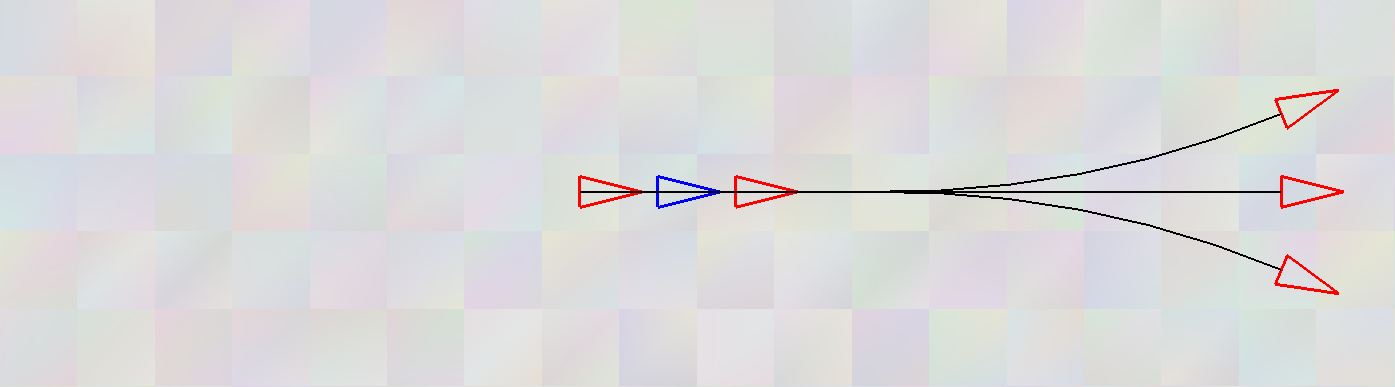
\includegraphics[width=0.2\textwidth]{unicycle.png}
%    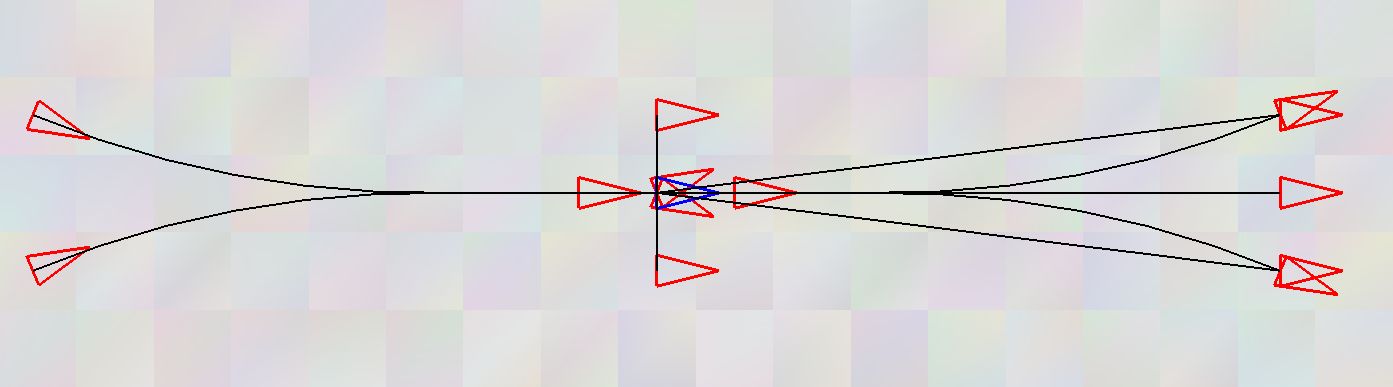
\includegraphics[width=0.2\textwidth]{pr2.png}\\
%    \caption{Motion primitives for unicycle (left) and a PR2 robot (right). \comment{If there are nice pictures for the motion primitives, that would be much better}}
%    \label{fig:motion-primitives}
%\end{figure}


Bartak et al.~\shortcite{bartak2018aScheduling} proposed a scheduling-based approach for \mapf on weighted graphs, and Walker et al.~\shortcite{walker2018extended} proposed a variant of the Increasing Cost Tree Search (ICTS) algorithm. Yakovlev and Andreychuk~\shortcite{yakovlev2017any} proposed a hybrid of the SIPP algorithm~\cite{phillips2011sipp} and prioritized planning for weighted graphs.

The types of weighted graphs that have been used in MAPF reseach so far include:
\begin{itemize}
    \item \textbf{MAPF in $2^k$-neighbor grids.}\footnote{Such grids are also referred to as $2^k$-connected grids.} Such maps are a restricted form of weighted graphs in which every vertex represents a cell in a two-dimensional grid. The move actions of an agent in a cell are all its $2^k$ neighboring cells, where $k$ is a parameter.
Costs are based on Euclidean distance, therefore when $k>2$, this introduces actions with different costs. For example, in an 8-neighbor grid a diagonal move costs $\sqrt{2}$ while a move in one of the cardinal directions costs 1. Figure~\ref{fig:k-neighborhood} shows the possible move actions in $2^k$-neighbor grids for $k=2, 3, 4,$ and $5$.

%\comment{Roni: maybe we can add a figure of a $2^k$ neighborhood here?}\comment{Thayne: Added figures and reference for $2^k$ grids}\comment{Roni: prefect - TNX!}

    \item \textbf{MAPF in Euclidean space.}
\mapf in Euclidean space is a generalization of \mapf in which every node in $G$ represents a Euclidean point ($x,y$), and the edges represent allowed move actions. Such settings arise, for example, when the underlying graph is a roadmap generated for a continuous Euclidean environment \cite{khatib1986real,wagner2012probabilistic}.
%\comment{Roni: if anyone can add a reference here, that'd be great}\comment{Thayne: Added two refs here.}

\end{itemize}

%\comment{Roni: anyone has a published paper to cite here? I got a paper with this, but it is not published yet}
%\comment{Roni: I am not familiar with other types of MAPF on weighted graphs. So please add what I am missing}

\subsection{Feasibility Rules}

The definition of a valid solution used in classical MAPF -- no conflicts -- is just one
type of solution requirement.
%We refer to the form of \emph{feasibility rule} known as the \emph{exclusion rule}~\cite{redacted2019generalizing}. MAPF can be solved with more feasibility rules beyond the exclusion rule.
We use the term \emph{feasibility rule} to refer to a requirement over a \mapf solution. Other \mapf feasibility rules have been suggested.

\begin{itemize}
\item \textbf{Robustness rules.} These are rules designed to ensure that a \mapf solution considers inadvertent delays in execution. A \emph{k-robust} MAPF plan builds in a sufficient buffer for agents to be delayed up to $k$ time steps without resulting in a conflict~\cite{atzmon2018robust}.
When the probability of future delays is known, robustness rules can require that the probability an agent will conflict during execution is lower than a given bound~\cite{wagner2017path} or be combined with execution policies to guarantee a conflict-free execution \cite{MaAAAI17}.

\item \textbf{Formation rules.} These are restrictions over the allowed move actions of an agent that depend on the location of the other agents but are not related to collisions. For example, restrictions intended for the agents to maintain a specified formation~\cite{barel2017come}, or to maintain a communication link with a set of neighboring agents~\cite{stump2011visibility,gilboa2006distributed}.

\end{itemize}


%Another feasibility rule raised in the context of \mapf is \emph{robustness}~\cite{atzmon2018robust}, which is the requirement that agents' paths must build in the possibility for inadvertent delays in execution. A \emph{k-robust} MAPF plan builds in a sufficient buffer for agents to be delayed up to $k$ time steps without resulting in a conflict.
%Additional feasibility rules include formation maintenance, rendezvous, clustering~\cite{barel2017come} and communications link maintenance~\cite{stump2011visibility,gilboa2006distributed} have also been explored, but many others are possible and remain an open question for MAPF research.

%\comment{Thayne: I think the concept of additional feasibility rules is a good notion to add to this paper...}\comment{Roni: Added}




\subsection{From Pathfinding to Motion Planning}
In classical MAPF, agents are assumed to occupy exactly one vertex, in a sense having no volume, no shape, and move at constant speed. By contrast, motion planning algorithms directly consider these  properties. There, an agent is situated at each time step in a \emph{configuration} instead of only a vertex, where a configuration specifies the agent's location, orientation, velocity, etc, and an edge between configurations represents kinematic motion. Several notable \mapf variants are steps towards closing this gap between classical \mapf and motion planning. %represent a middle ground between classical \mapf and MAMP.

\subsubsection{\mapf with large agents.}
Some \mapf research considered agents with a specific geometric shape and volume~\cite{li2019multi,walker2018extended,yakovlev2017any,thomas2015extended}. The fact that agents have volume raises questions about how they are situated in the underlying graph $G$ and how they move in it. In particular, if an agent is located in one vertex, it may prohibit other agents from occupying nearby vertices.
Similarly, if an agent moves along an edge it may prohibit other agents from moving along intersecting edges or staying at vertices that are too close to the edge. This may introduce new types of conflicts, such as vertex-to-vertex, edge-to-edge, and edge-to-vertex conflicts \cite{honig2018trajectory}.
%\comment{Roni: to elaborate?}
%can introduce new types of conflicts. In particular, collisions may occur between agents located in different vertices or traversing different edges. a pair of agents occupying different vertices may can occupy at different vertices but still have a conflict. means that more types of conflicts are relevant. The shape of the agents may be such that a pair of agents can occupy different vertices but still have a conflict. Similarly, different edges may give rise to an edge conflict, and an agent traversing an edge may conflict with a different agent occupying vertex. [[AF: the above is a little vauge. The most important issue is how agents are placed in the graph and that a conflict is where their shapes overlap]]


Several approaches for solving \mapf with large agents have appeared in the literature, including a CBS-based approach~\cite{li2019multi}, an ICTS-based approach~\cite{walker2018extended}, and a prioritized planning approach~\cite{yakovlev2017any}. A special case of agents with volume is the \emph{convoy} setting, in which agents occupy a string of vertices and their connecting edges \cite{thomas2015extended}.

\subsubsection{\mapf with kinematic constraints.}
Other \mapf research considered kinematic constraints over agents' move actions~\cite{honig2017summary,walker17hierarchical}. That is, the move actions an agent can perform depend not only on its current location, but also on state parameters such as velocity and orientation. A by-product of such constraints is that the underlying graph becomes directed, as there may be edges that can only be passable in one direction due to kinematic constraints of the agent.  MAPF-POST, as an example, is a \mapf algorithm that considers these kinematic constraints by post-processing a solution created by a \mapf algorithm. There is also a reduction-based approach that assumes rotation actions as a half way to kinematic constraints~\cite{BartakIBERAMIA18}.



%\subsection{Multi-Agent Motion Planning}
%\comment{Roni: below
%\comment{Roni: TODO: Think about how I think I'll move all that's below to a bullet in the above list titled ``\mapf in Configuration Space'', and lose the formal part. Thoughts on this? a reference on MAPF in such a space will also be helpful}

%The Multi-Agent Motion Planning (MAMP) problem is a richer formulation that is applicable to MAPF on weighted graphs and agents with volumes. Unlike the above formulations, the MAMP problem is posed on states instead of locations. A state specifies discretized values of an agent's location, orientation, velocity, etc. An edge represents a kinodynamically feasible motion with an arbitrary duration. The sequence of motions in a feasible plan leads an agent from its start state to its goal state. An agent is allowed to take any geometric shape, implicitly specified by a set of occupied cells.\comment{Liron: I don't know if you want to keep the formal definition below, feel free to keep just parts of it.}

%We formally define the MAMP problem as follows. We are given an environment represented by a list of cells $\mathcal{C}$. We are given agents $1, \ldots, K$, each with an associated graph $G^j=(V^j,E^j)$ and start and goal vertices, $s^j, g^j \in V^j$. Each vertex $s \in V^j$ represents a \emph{state} and is associated with a list of cells $\{c^s_1, \ldots, c^s_{m(s)} \} \subseteq \mathcal{C} $ occupied by the agent while at $s$. Each edge $e \in E^j$ represents a \emph{motion} and has an associated weight, $w(e) > 0$, that represents its duration. $e$ is also associated with a multiset of cells $\{c^e_{1}, \ldots, c^e_{m(e)}\} \subseteq \mathcal{C}$. Each cell $c^e_i$ is associated with a time interval $[lb^e_i, ub^e_i]$ during which it is swept by $e$ after the beginning of its execution. Thus $\min_{1 \leq i \leq m(e)} lb^e_i = 0$ and $\max_{1 \leq i \leq m(e)} ub^e_i = w(e)$.

%A sequence $\pi^j = \{ \langle e^j_1,t^j_1 \rangle, \ldots, \langle e^j_{T_j},t^j_{T_j} \rangle \}$ is a plan for agent $j$, where $e^j_i=(s^j_{i-1},s^j_i) \in E^j$ and $t^j_i \geq 0$ is the beginning time of the execution of $e^j_i$. $\pi^j$ is \emph{feasible} if and only if $e^j_1 \ldots, e^j_{T_j}$ is an $s^j$-$g^j$ path in $G^j$ and, for all $i \in \{2, \ldots, T_j\}$, $t^j_{i} \geq t^j_{i-1} + w(e^j_{i-1})$. This means that agent $j$ waits at state $s^j_{i-1}$ and therefore occupies cells $\{c^s_1, \ldots, c^s_{m(s)} \}$ for $s=s^j_{i-1}$ during the time interval $[t^j_{i-1} + w(e^j_{i-1}), t^j_{i}]$.\footnote{Waiting can be conditioned on the velocity being zero.} We assume that agent $j$ occupies $\{c^s_1, \ldots, c^s_{m(s)} \}$ for $s=g^j$ during the time interval $[t^j_{T_j} + w(e^j_{T_j}),\infty]$. The travel time of agent $j$ in $\pi^j$ is given by $t^j_{T_j} + w(e^j_{T_j})$. A \emph{collision} between two agents occurs if the time intervals in which they sweep or occupy the same cell overlap. A \emph{solution} to the MAMP problem is a set of feasible plans such that no two agents collide.





\subsection{Tasks and Agents}

In classical MAPF, each agent has one task - to get it to its target. Several extensions have been made in the MAPF literature in which agents may be assigned more than one target.

\subsubsection{Anonymous \mapf.}
In this \mapf variant, the objective is to move the agents to a set of target vertices, but it does not matter which agent reaches which target~\cite{kloder2006path,yu2013multi}.
Another way to view this \mapf variant is as a \mapf problem in which every agent can be assigned to any target, but it has to be a one-to-one mapping between agents and targets.

\subsubsection{Colored \mapf.}
This \mapf variant is a generalization of anonymous \mapf in which agents are grouped into teams, and every team has a set of targets. The objective is to move the agents in each team to their targets~\cite{ma2016optimal,solovey2014k}. Another way to view this \mapf variant is as a \mapf problem in which every agent can be assigned to targets only from the set of targets designated for its team.

One can generalize colored \mapf even further, assigning a target and an agent to multiple teams.
%to the  In this \mapf variant, every agents and every goals is colored. Any agent can go to any target that    \item \textbf{$k$-Color MAPF.}      In this MAPF variants, agents and goals are colored and any agent may be assigned to any goal of the same color.\cite{ma2016optimal,solovey2014k}     \item \textbf{Typed MAPF.}     This MAPF variant is a generalization of $k$-Color MAPF. Here, each agent and goal can have several types. Any agent can be assigned to a goal only if they share a common type.   \end{itemize}


\subsubsection{Online MAPF.}
In \emph{online \mapf}, a sequence of \mapf problems are solved on the same graph. This setting has also been called ``Lifelong MAPF''~\cite{MaAAMAS17,MaAAAI19b}. Online \mapf problems can be classified as follows.
\begin{itemize}
    \item \textbf{Warehouse model.} This is the setting where a fixed set of agents solve a \mapf problem, but after an agent finds a target, it may be tasked to go to a different target~\cite{MaAAAI19b}. This setting is inspired by \mapf for autonomous warehouses.
    \item \textbf{Intersection model.} This is the setting where new agents may appear, and each agent has one task -- to reach its target~\cite{svancara2019online}. This setting is inspired by autonomous vehicles entering and exiting intersections~\cite{dresner2008multiagent}.
\end{itemize}
Of course, hybrid models in which an agent can receive a new task when it reaches its target and new agents can appear over time is also possible.

\section{Benchmarks}

% Why benchmarks
In this section, we describe how classical \mapf algorithms have been evaluated, suggest an organized benchmark for this purpose, and point to other relevant benchmark suites.

% Common approach: choose a grid, then choose start and goal locations
\subsection{Characteristics of a \mapf Benchmark}
A \mapf problem is defined by a graph and a set of source and target vertices. As such, a benchmark for \mapf includes a set of graphs, and for every graph a set of sets of source and target vertices.
%The type of graph most commonly used is a 4-connected grid.
\subsubsection{Graphs for evaluating \mapf algorithms.}
The types of maps commonly used in prior work include:
\begin{itemize}
    \item \textbf{Dragon Age Origins (DAO) maps.} These are grids taken from the game Dragon Age Origin and are publicly available in Sturtevant's \texttt{movingai.com}  repository~\cite{sturtevant2012benchmarks}.
    These grids are relatively large and open, where some grids are as large as a $1000\times 1000$ and more.

    \item \textbf{Open $N\times N$ grids.} These are $N\times N$ grids, where common values of $N$ are 8, 16, and 32. Such grids allow experiments in which the ratio of agents to space or \emph{agent density} is high, having fewer vertices without an agent in them.

    \item \textbf{$N\times N$ grids with random obstacles.} These are  $N\times N$ grids, where a set of grid cells are randomly  selected and are considered to be impassable (obstacles)~\cite{standley2010finding}.

    \item \textbf{Warehouse grids.} Inspired by real-world autonomous warehouse applications, recent \mapf papers also experimented with grids shaped to be similar to an automated warehouse, with long corridors~\cite{MaAAMAS17,cohen2018anytime}. Figure~\ref{fig:warehouse} shows an illustration of a warehouse grid taken from~\cite{cohen2018anytime}.
\end{itemize}
%\comment{Jiaoyang: Maybe we also want to include some warehouse maps and general graphs.}
%\comment{Liron: I agree with Jiaoyang. Warehouse domains are interesting because the start and goal locations are not evenly distributed across the map. I'm happy to contribute map or instances.}
%\comment{Roni: good idea, if you can add text from your paper that describes Warehouse, that'd be great}

\comment{Roni: I wonder if we should add roadmaps. Thoughts?}



\subsection{Sources and targets assignments}
\label{sec:source-target-assignment}

After choosing a type of map, one needs to set the agents' source and target vertices.
Several methods for setting agents' sources and targets have been used in the literature, including:

\begin{itemize}
    \item \textbf{Random.} Setting the source and target vertices by randomly choosing vertices and making sure there is a path in the graph between them.
    \item \textbf{Clustered.} Setting the first agent's source and target by randomly choosing vertices in the graph. Setting the sources and targets of all others agents to be with distance of at most $r$ from the first agent's source and target, respectively, where $r$ is a parameter.
%    \item \textbf{Uni} \comment{Roni: Nathan, can you explain a bit on this?}
    \item \textbf{Designated.} Setting the source of each agent by randomly choosing from a designated set of possible source vertices, and setting the target of each agent similarly by choosing from a set designated set of possible target vertices.
\end{itemize}


% Elaboration and where it was used
\emph{Random} assignment is probably the most common in the literature. The \emph{clustered} assignment method has been used to make \mapf problems more challenging.\comment{Roni: TODO: Add a reference of someone doing this}
The \emph{designated} assignment method has been used in prior work in an effort to simulate automated warehouses~\cite{DBLP:conf/socs/CohenUK15,MaAAAI19a,MaAAAI19b} and autonomous vehicles in intersections~\cite{svancara2019online}. In an automated warehouse, there are often humans situated in specific locations to package the delivered bin and most tasks deliver a package to, or retrieve a package from, a human in these locations. In a setting with autonomous  vehicles driving in and out of an intersection, the designated sources and targets are the intersection end points~\cite{svancara2019online}.




\begin{figure}[tb]
    \centering
    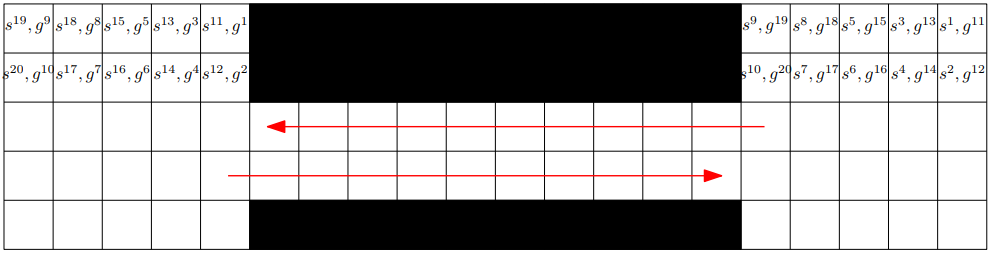
\includegraphics[width=\columnwidth]{designated.PNG}
    \caption{An example of a designated method for setting sources and targets, taken from~\cite{DBLP:conf/socs/CohenUK15}. They chose randomly a source from the open space on the left and a target from the open space on the right for 25\% of the agents, and chose sources and targets from open spaces on the right and left, respectively, for the rest of the agents.}
    % \label{fig:designated}
\end{figure}

\begin{figure}[tb]
    \centering
    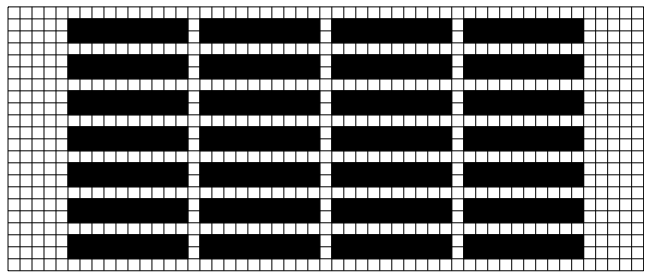
\includegraphics[width=\columnwidth]{warehouse.PNG}
    \caption{Illustration of a warehouse grid~\cite{CWKKCS:AAMAS:18}.}
    % \label{fig:warehouse}
\end{figure}



% Description of benchmark
\subsection{Publicly Available \mapf Benchmarks}

We describe here two publicly available benchmarks for \mapf research, the first of which is a new benchmark set described for the first time in this paper.

\subsubsection{Grid-based \mapf.}

\begin{figure}[tb]
    \centering
    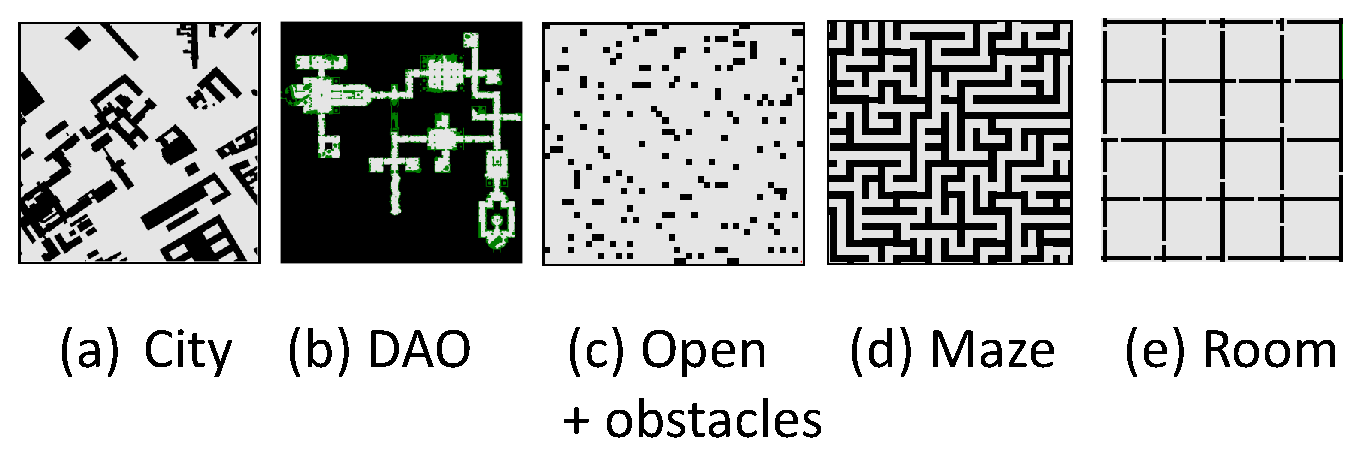
\includegraphics[width=\columnwidth]{map-types.pdf}
    \caption{An example of a map from each type of maps available in the grid \mapf benchmark.}
    \label{fig:map-types}
\end{figure}

% Please add the following required packages to your document preamble:
% \usepackage{booktabs}
% \usepackage{multirow}
\begin{table}
\resizebox{\columnwidth}{!}{
\begin{tabular}{@{}llcrrrr@{}}
\toprule
\multicolumn{1}{l}{Type}                                                   & \multicolumn{1}{l}{Map} & Size       & \multicolumn{1}{c}{Problems} & \multicolumn{1}{c}{Solved} & \multicolumn{1}{c}{Min} & \multicolumn{1}{c}{Max} \\ \midrule
\multirow{3}{*}{City}                                                      & Berlin\_1\_256          & 256 X 256  & 25000    & 892    & 4                       & 52                      \\
                                                                           & Boston\_0\_256          & 256 X 256  & 25000    & 718    & 13                      & 47                      \\
                                                                           & Paris\_1\_256           & 256 X 256  & 25000    & 805    & 3                      & 47                      \\
\midrule \multirow{6}{*}{DAO}                                                       & brc202d                 & 481 X 530  & 25000    & 252    & 2                       & 22                      \\
                                                                           & den312d                 & 81 X 65    & 25000    & 577    & 7                      & 36                      \\
                                                                           & den520d                 & 257 X 256  & 25000    & 661    & 5                      & 47                      \\
                                                                           & lak303d                 & 194 X 194  & 25000    & 377    & 8                      & 27                      \\
                                                                           & orz900d                 & 656 X 1491 & 25000    & 162    & 2                       & 12                       \\
                                                                           & ost003d                 & 194 X 194  & 25000    & 535    & 7                      & 37                      \\
\midrule \multirow{4}{*}{\begin{tabular}[c]{@{}l@{}}Dragon \\ Age 2\end{tabular}}   & ht\_chantry             & 141 X 162  & 25000    & 513    & 11                      & 35                      \\
                                                                           & ht\_mansion\_n          & 270 X 133  & 25000    & 795    & 17                      & 42                      \\
                                                                           & w\_woundedcoast         & 578 X 642  & 25000    & 336    & 6                       & 22                      \\
                                                                           & lt\_gallowstemplar\_n   & 180 X 251  & 25000    & 493    & 10                       & 32                      \\
\midrule \multirow{4}{*}{Open}                                                      &                                                                             empty-8-8               & 8 X 8      & 800      & 528    & 18                      & 25                      \\
& empty-16-16             & 16 X 16    & 3200     & 840    & 15                       & 52                      \\
                                                                           & empty-32-32             & 32 X 32    & 12800    & 1190   & 12                       & 81                      \\
                                                                           & empty-48-48             & 48 X 48    & 25000    & 1349   & 18                      & 118                     \\

\midrule \multirow{4}{*}{\begin{tabular}[c]{@{}l@{}}Open+\\ obstacles\end{tabular}} & random-32-32-10         & 32 X 32    & 11525    & 1027   & 15                      & 68                      \\
                                                                           & random-32-32-20         & 32 X 32    & 10225    & 862    & 15                      & 46                      \\
                                                                           & random-64-64-10         & 64 X 64    & 25000    & 1450   & 24                      & 87                      \\
                                                                           & random-64-64-20         & 64 X 64    & 25000    & 1078   & 10                      & 64                      \\
\midrule \multirow{4}{*}{Maze}                                                                           & maze-32-32-2            & 32 X 32    & 8325     & 327    & 8                       & 17                      \\
                                                                           & maze-32-32-4            & 32 X 32    & 9875     & 317    & 4                       & 23                      \\
                                                                           & maze-128-128-10         & 128 X 128  & 25000    & 272    & 5                       & 20                      \\
                                                                           & maze-128-128-2          & 128 X 128  & 25000    & 178    & 4                       & 15                      \\

\midrule \multirow{3}{*}{Room}                                                      & room-32-32-4            & 32 X 32    & 12800    & 469    & 10                      & 26                      \\
%                                                                           & room-32-32-8            & 32 X 32    & 10100    & -    & -                      & -                      \\
                                                                           & room-64-64-16           & 64 X 64    & 25000    & 629    & 12                      & 45                      \\
                                                                           & room-64-64-8            & 64 X 64    & 25000    & 360    & 8                       & 24                      \\ \bottomrule
\end{tabular}
}
\caption{Results for running ICBS with a timeout of 30 seconds on the grid \mapf benchmark.}
\label{tab:results}
\end{table}


This publicly available\footnote{\url{https://movingai.com/benchmarks/mapf.html}} benchmark consists of 24 maps taken from (1) maps of real cities, (2) the video games Dragon Age Origins and Dragon Age 2, (3) open grids with and without random obstacles, (4) maze-like grids, and (5) room-like grids. All maps were taken from the MovingAI pathfinding repository~\cite{sturtevant2012benchmarks}.\footnote{\url{https://movingai.com/benchmarks/grids.html}}
Figure~\ref{fig:map-types} shows an example of a map from each of these types,
and Table~\ref{tab:results} shows the dimensions of these maps.

% Scenario generated
Every map has 25 \emph{scenarios}.
Every scenario has a list of source and target vertices that
were set using a variant of the random method (see Section~\ref{sec:source-target-assignment}) All points in the largest reachable region of each map were randomly paired, and then the first 1000 problems were put into the scenario. Thus, one can create a set of \mapf problems from each scenario by choosing any subset of source and target vertices.

% Intended usage
We propose using this benchmark in the following way.
For a chosen \mapf algorithm, map type, and scenario,
try to solve as many agents as possible in each scenario, adding them in consecutive order. That is, start by creating a \mapf problem of two agents, using the first two source-target pairs associated with the chosen scenario,
and run the \mapf algorithm of choice to solve this problem.
If the algorithm of choice successfully solves this \mapf problem in reasonable time, create a new \mapf problem with 3 agents by using the first three source-target pairs of that scenario and try to solve it with the \mapf algorithm of choice. This continues iteratively until the algorithm of choice cannot solve the created \mapf problem in reasonable time. An evaluated algorithm can then report, for every scenario, the maximal number of agents it was able to solve in reasonable time.

\comment{Nathan: Please use the terminology from this paper to describe the ICBS settings used for this experiment.}
To provide a baseline for comparison, we performed this evaluation process using ICBS~\cite{boyarski2015icbs}. Using the terminology introduced in this paper, our setting was a classical \mapf setting on a 4-neighbor grid
where
(1) edge, vertex, and swapping conflicts were forbidden,
(2) following and cycle conflicts were allowed,
(3) the objective was the sum of costs, and
(4) the agent behavior at target is stay at target.

Table~\ref{tab:results} shows the result of this evaluation. We set 30 seconds as the runtime limit.
The different rows correspond to different maps.
The ``Size'' column reports the number of rows and columns in each map.
The ``Problems'' column reports the number of problems available for each map.
Note that this number is aggregated over the 25 scenarios, where the number of problems available in a scenario is the number of source-target pairs defined for it. \comment{Roni: is the above clear? Nathan: Mostly - I don't see a good way to improve it.}
The ``Solved'' column reports the number of problems solved by ICBS under the specified time limit (30 seconds). As can be seen, while ICBS is able to solve many problems, the problems in this benchmark are complex enough so that there are many problems that cannot be solved by ICBS in the allotted time. Thus, the problems in this grid \mapf benchmark are hard enough to pose a challenge for contemporary \mapf solvers.


Table~\ref{tab:results} has two additional columns - ``Min'' and ``Max''. These columns report the maximal number of agents solved by ICBS
in the scenario in which this number was smallest (``Min'') and when it was largest (``Max''). For example, the ``Min'' value for map \texttt{brc202d} is 2 and the ``Max'' is  22. This means there exists a scenario for this map in which ICBS were able to solve at most 2 agents before reaching a timeout,
and there is a different scenario for this map in which ICBS were able to solve up to 22 agents. We report these values to show the diversity in difficulty between the scenarios of the same map.

\subsubsection{Asprilo.}


\begin{figure}[tb]
    \centering
    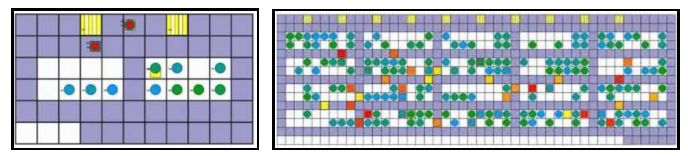
\includegraphics[width=\columnwidth]{asprilo_cropped.pdf}
    \caption{Two scenarios from the Asprilo framework. The left figure is a full warehouse scenario, which includes moving bins from one place to another. The right figure is a movement-only scenario, which corresponds to a classical \mapf problem.}
    \label{fig:asprilo}
\end{figure}

%\comment{TODO: Also mention ASPRILLO}
An additional tool that is useful for \mapf research is Asprilo.
Asprilo is a publicly available framework for simulating an automated warehouse~\cite{martin2018experimenting}. It includes tools for defining and generating standard automated warehouse planning problems, and tools for verifying and visualizing plans that solve these problems.

The type of planning problems supported by Asprilo includes problems in which robots are tasked to pick up and deliver bins in the warehouse from one place to another. These scenarios are grouped into different \emph{domains}, representing different types of problems. Of interest to the \mapf community in particular is domain $M$, which basically represents \mapf problems. Thus, one can use problems from this domain as a benchmark for \mapf algorithms.
Figure~\ref{fig:asprilo} shows two scenarios from Asprilo. The scenario depicted on the left side is a full warehouse scenario, where the agents are tasked to move bins from one place to another. The scenario on the right side is a movement-only scenario, i.e., a classical \mapf problem.
Details on ASPRILO can be found in~\cite{martin2018experimenting}, as well as the project's website.\footnote{\url{https://asprilo.github.io}}

\section{Conclusion}
In the first part of this paper, we defined common assumptions in the ``classical'' Multi-Agent Pathfinding (\mapf) problem and discuss the relationships between them. Then, we defined notable extensions to classical \mapf that were previously published.
In the second part of this paper, we introduced a new suite of \mapf benchmark problems and point to another set of \mapf benchmark problems.
Both parts of this paper are intended to propose a common language, terminology, and experimental setting for \mapf research. It is our hope that future \mapf researchers will follow our terminology and find these benchmarks useful.

\section{Acknowledgments}
This research is supported by ISF grants no. 210/17 to Roni Stern and \#844/17 to Ariel Felner and Eyal Shimony, by BSF grant \#2017692 and by NSF grant \#1815660. %Marek


\vskip 0.2in
Ab fuga veniam numquam quae explicabo temporibus esse repudiandae tempora doloremque, esse rem ab rerum voluptatibus sit odit perferendis, magnam pariatur saepe itaque officia minima?Tempore fugit pariatur at veniam, cum enim vero a consequuntur labore velit, aperiam non sed adipisci ad debitis ratione cumque beatae?Quasi ut adipisci saepe eaque doloremque est voluptate quaerat, quos facilis  impedit omnis.\clearpage
\bibliography{library}
\bibliographystyle{aaai}

\end{document}